\documentclass[12pt]{article}

\usepackage[utf8]{inputenc}
\usepackage{latexsym,amsfonts,amssymb,amsthm,amsmath}
\usepackage[T1]{fontenc}
\usepackage{titling}
\usepackage{graphicx}
\usepackage{url}

\setlength{\droptitle}{-4em}  
\setlength{\parindent}{0in}
\setlength{\oddsidemargin}{0in}
\setlength{\textwidth}{6.5in}
\setlength{\textheight}{8.8in}
\setlength{\topmargin}{0in}
\setlength{\headheight}{0pt}

\title{Computación Concurrente. Práctica 1.}

\author{
    Martínez Mejía Eduardo \\
    a
}

\date{27 de Agosto de 2026}

\begin{document}

\maketitle

\vspace{0.5cm}

\subsection*{1. https://www.evanjones.ca/software/threading-linus-msg.html.\\
Comparte
en máximo 4 líneas de computadora a qué se refiere Linus Torvalds con un contexto de ejecución
y cómo se relaciona con la definición en la sección 1 de esta práctica.}

Es un conjunto de estados de la computadora asociados a una tarea. Verlo así permite dejar de ver sólo hilos y procesos  como varios caminos bifurcados actuando sobre un mismo plan, sino ver módulos con datos propios que pueden manejar y compartir según se requiera, sin la limitación de depender completamente de un padre, teniendo total libertad de ejecución.
\\


\subsection*{2. ¿Cuántos hilos tiene disponibles tu computadora?\\
Ejecuta \textit{Runtime.getRuntime().availableProcessors()}, si son más de uno en el equipo escriban el
de cada uno.}

\begin{itemize}
    \item \textbf{Eduardo}: 
        \\ 
\includegraphics[width=15cm]{imagenes/EduardoP2.png}
    
    \item \textbf{Ricardo}:
        \\ 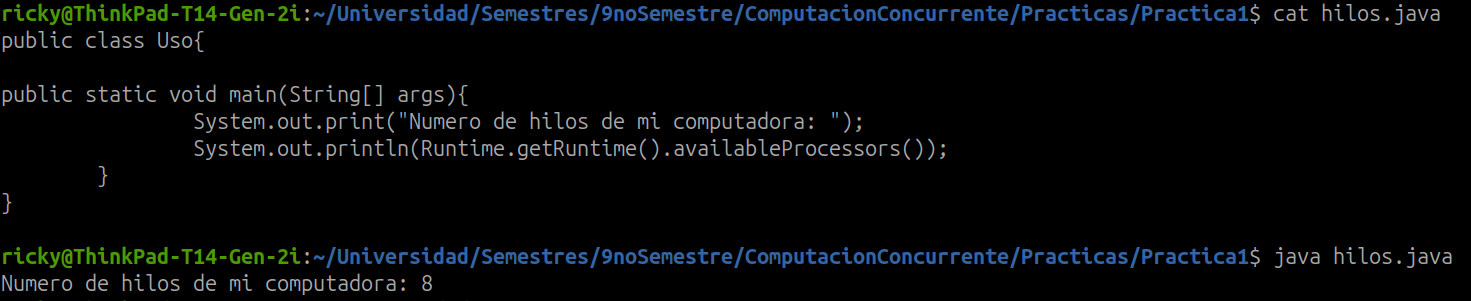
\includegraphics[width=15cm]{imagenes/num-hilos-richard.png}
    
    \item \textbf{Hazel}: 
        \\ 
\includegraphics[width=5cm]{imagenes/Hazel_1.png}
    
\end{itemize}
\\


\subsection*{3. Revisa el programa \textit{Determinante} concurrente y responde ¿Cuánto tiempo tarda en ejecutarse?.}

\begin{itemize}
    \item \textbf{Eduardo}: \\
\includegraphics[width=16cm]{imagenes/EduardoP3.png}
    
    \item \textbf{Ricardo}: 
        \\ 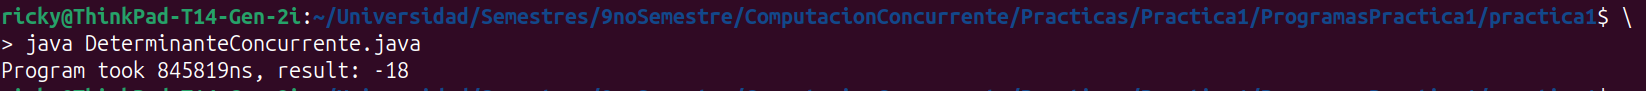
\includegraphics[width=16cm]{imagenes/determinante-concurrente-richard.png}
    
    \item \textbf{Hazel}: 
        \\ 
\includegraphics[width=7cm]{imagenes/Hazel_2.png}
\end{itemize}
\\


\subsection*{4. El programa \textit{Determinante} concurrente está implementado extendiendo la clase \textit{Thread}. Implementa
el programa utilizando la interfaz \textit{Runnable}.}

Partiendo del programa \textit{Determinante}, cambiamos la definición de la clase para que implemente \textit{Runnable}, cambiando su nombre a  \textit{DeterminanteConcurrenteRunnable} para distinguirla.
\\
Como cada hilo que necesitamos para dividir cada conjunto de multiplicaciones a  efectuar al aplicar la regla de \textit{Sarrus}, debemos crear los objetos runnable necesarios, en este caso son 6 al ser una matriz $3x3$, con lo que le podemos pasar a cada uno los valores de la matriz con los que debe operar.
\\
De aquí partimos para crear un thread para cada runnable y comenzar la ejecución, siguendo exactamente las mismas instrucciones que cuando se decidió extender \textit{Thread}.


\\


\subsection*{5. Implementa el programa \textit{Determinante} concurrente de forma secuencial.}
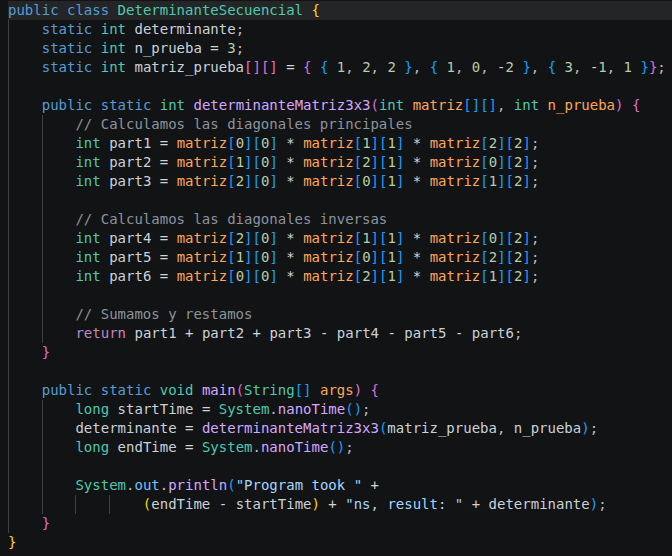
\includegraphics[width=10cm]{imagenes/DeterminanteSec.png}
\begin{enumerate}
    \item Para calcular el determinante de una matriz 3x3, primero calculamos el producto de las tres diagonales principles

    \item posteriormente, calculamos las diagonales secundarias 

    \item Tomamos los primeros tres resultados y los sumamos

    \item Y por ultimo, a esa suma le restamos los ultimos tres resultados
\end{enumerate}
\\


\subsection*{6. Implementa del programa \textit{Determinante} concurrente para dos hilos (en vez de seis).}

El código fuente es el del archivo \textit{DeterminanteConcurrenteDosHilos.java.} 

\begin{enumerate}
    \item Nos basamos en el archivo que tenía 6 hilos.

    \item Dividimos el trabajo de cálculo en 2 hilos, ahora cada hilo iba a trabajar con 9 operandos. Dividimos la resta final del cálculo del determinante en dos pasos. Cada hilo ahora sólo multiplica sus 9 parámetros.

    \item Finalmente se resta el producto de cada hilo para obtener el determinante. 
\end{enumerate}


\subsection*{7. Compara las 3 implementaciones: el programa \textit{Determinante} concurrente para dos hilos, para seis hilos y el programa secuencial. 
\\ Responde: ¿A qué se debe el orden en el que se ordenan los
tiempos de ejecución de cada programa?}

Los tiempos de ejecución de las diferentes versiones del programa resultaron ser, de mayor a menor las siguientes:
\begin{itemize}
    \item Secuencial
    \item Concurrente de 2 hilos
    \item Concurrente de 6 hilos
\end{itemize}

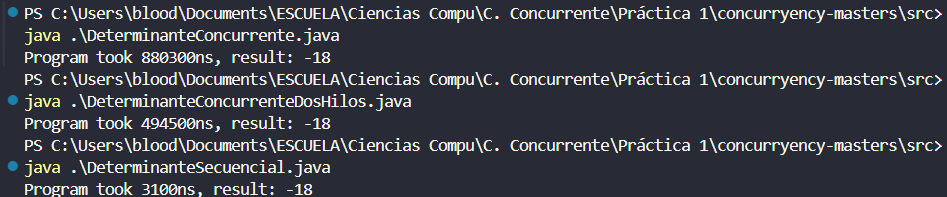
\includegraphics[width=16cm]{imagenes/TiemposDeterminantes.png}

Analizando el algoritmo base nos podemos dar cuenta de que realmente el calcular la determinante de una matriz $3x3$ requiere de pocas operaciones, por lo que podemos pensar que el aumento de tiempo de ejecución que observamos se debe al costo de la creación e inicialización  de cada hilo, lo que agrega tiempo extra, por lo que mientras más hilos, más tiempo tomamos. Podemos entonces ver que en este problema específico no ganamos velocidad real en la práctica.
\\


\subsection*{8. Si utilizas la Ley de Amdahl entre el programa \textit{Determinante} concurrente para dos hilos y el programa secuencial. ¿El resultado es mayor o menor a 1? ¿Por qué?.}

Al ejecutar el programa secuencial, éste tardo $a=3501 ns$, y al ejecutar el de dos hilos tardó $b=896995 ns$. Es decir, $a/b$ es menor a 1. Por lo tanto, no hay aceleración con dos hilos que con secuencial. Esto probablemente se debe a que estos cálculos son muy simples y rápidos para un procesador normal, y tarda menos que todo el proceso de crear hilos.
\\


\subsection*{9. Describe con tus propias palabras en máximo dos líneas para qué sirve el método \textit{join()}. Si no
utilizas el método \textit{join()} en \textit{Determinante Concurrente}, ¿sigue funcionando?}

Detiene al hilo principal para que los hilos a los que llama terminen su trabajo antes de continuar, siendo útil para juntar sus resultados.
\\
\\
Si se comentan todos los \textit{join()} deja de funcionar y el resultado arroja 0, pues cada hilo termina después del principal \textit{determinanteMatriz3x3}, y al instante se suman los valores \textit{partial} de cada hilo, que se inicializaron en 0. 
\\


\end{document}

